\documentclass[]{article}
\usepackage[left=3.8cm, right=3.8cm, top=2.50cm, bottom=2.50cm]{geometry}
\usepackage{lipsum}
% \usepackage{todonotes}
\usepackage[disable]{todonotes}
\usepackage{graphicx}
\usepackage{caption}
\usepackage{subcaption}
\usepackage[]{threeparttable}
\usepackage[normalem]{ulem}
\usepackage{url}
\usepackage{listings}
\usepackage{multirow}

\usepackage[utf8]{inputenc}

\setuptodonotes{size=tiny, color=blue!30}

\title{The Proof of Reputation Protocol \small{draft}}
\author{Ki Foundation}
\date{October 2019}

\begin{document}
\maketitle
\begin{abstract}
The consensus mechanism is a pillar of any blockchain. It guarantees the existence, at any instant, of a unique valid state of the system across the majority of the nodes. In this document we describe the Proof of Reputation protocol, a novel consensus mechanism for blockchain environments. It leverages the behavioral trust of the nodes and their stake in order to provide a decentralized and secure validation process while reducing the plutocracy and centralization tendency found in the existing consensus mechanisms.    
\end{abstract}
\section{Introduction}
\label{sec:intro}
Fostered by the growing need for more secure and scalable data management and transaction systems, decentralized applications and solutions have been emerging, in the last decade, at a firm and fast pace. These, however, have struggled to reach the level of reliability that allows them to be adopted as large scale solutions. This is due to the lack of a trustworthy and powerful infrastructure, on which these systems can be deployed and run. Indeed, existent decentralized networks (also called consensus networks) rely on heterogeneous volunteer devices, which renders them subject to constant churn and resource pool unstablity. The Ki Foundation \todo{REF} proposes to tackle this problem by deploying a large fleet of its connected voice assistant, dubbed Domo\todo{REF}, to serve as a reliable and always available infrastructure for decentralized systems.

This hardware infrastructure is exploited and coordinated, in a decentralized fashion, through the Ki blockchain. Following a common approach, the Ki blockchain is maintained and secured by the effort of the connected nodes - be the Domos or any other node - which validate the transactions and forge confirmed blocks to the chain. In return, these "validators" are awarded a given amount\footnote{The reward scheme and the used inflationary policy are detailed is a separate document which can be found at: \url{link} }\todo{Add Link} of the blockchain native token called "Ki". To tackle the limitations of the common consensus mechanisms - which mainly includes: energy efficiency, plutocracy and privacy - the Ki blockchain utilizes a novel consensus protocol called the Proof of Reputation protocol (PoR). The latter inherits the speed and energy efficiency of the delegated Proof of Stake (dPoS) by adopting its delegation approach, and corrects its flaws i.e., the tendency to centralize and the validator churn, by leveraging the trust of the nodes and a random validator committee selection process.                  

This document describes the different components that constitutes the PoR protocol and delivers their technical details while motivating the made choices on both the theoritical and practical levels. It is structured as follows: in Section \ref{sec:overview}, an overview of the system architecture and its components is given. Then, these components are described in details in Section \ref{sec:behavior} (behavioral reputation), section \ref{sec:stake} (staking reputation) and Section \ref{sec:epoch} (reputation epochs). Finally, a brief review of the related works is provided in Section \ref{sec:related} before concluding the document in Section \ref{sec:conclusion}.

\section{An overview of PoR}
\label{sec:overview}
In this section, we motivate the creation of a new consensus protocol in the light of the limitations of state-of-the-art approaches which we briefly develop. We then provide a high level overview of the PoR protocol. 
\subsection{Motivation}

The Proof of Work (PoW) consensus protocol, while secure in its approach, is a largely centralizing factor within PoW networks, as the validation power is correlated to the expensive computational capacity dominated by the professional validators and the large mining pools. Moreover, it has a negative ecological footprint through it's large inefficient energy usage and is also not secure for smaller networks due to the generally low switching costs (consequently: every network at launch). Proof of Stake (PoS) consensus, while more energy-efficient, also leans towards centralization over time  as validation power is correlated to the validators' wealth (i.e. the validator token stake). Furthermore, it is vulnerable to nothing-at-stake attacks and suffers from an inability to efficiently scale.

The Delegated Proof of Stake (DPoS) consensus solves - theoretically - the majority of these problems thanks to its delegation process. In DPoS, users (a.k.a. delegators) vote to select ‘witnesses’ (a.k.a. delegates), who if they receive enough votes, earn the right to validate blocks for that round. Votes are weighted according to the size of each voter's stake. Unlike in PoS, a user does not need to own a large stake to be elected as a validator. Rather, votes from users with large stakes can result in users with relatively small stakes being elevated to the top tier of witnesses. Indeed, if the same witnesses are selected in each round, the validation process tends to become centralized, which compromises the integrity of the network and reduces the incentives for new validators to enter the market. Practically speaking, many DPoS based blockchains have converged over time to a quasi-fixed delegate list \todo{link to YP 2}. 

The limitations of the existent consensus protocols motivate the creation of a new secure protocol that is not solely correlated - directly or not - to the wealth of the validators and does not tend to concentrate the validation power in the hands of a fixed set of them. In the remainder of this document we explain how this limitation of dPoS can be tackled while maintaining the security and speed ensured by the community voting scheme.


\subsection{The PoR components}
\label{sec:components}
The block creation in a consensus network consists of two steps: selecting the block creator i.e., the validator, and validating the block. Hereafter, we describe how these two steps occur in PoR.   

\subsubsection{Validator list selection}
\label{sec:components:valsel}
The centralization problem in the state-of-the-art consensus mechanisms raises from the fact that they assesses the reliability of the validators, consequently their chance of validating blocks, by relying on one commitment criterion. That is the wealth, be it the computational power, the stake or the delegated stake. To solve this problem, one needs to identify and measure a complementary commitment criterion that allows to maintain the security guarantees on the blockchain while decoupling the validation chance from the bare wealth. The Proof of Reputation protocol leverages, beside their delegated stakes, the trust of the nodes in order to determine their reliability and compute their chance of validating blocks. This prevents the system from suffering from the plutocracy as the trust, as we will explain later, can be built by any node regardless their stake. During the validator list selection and to solve the centralization tendency problem\footnote{The centralization tendency is the tendency of a system, in a \textbf{practical} context, to concentrate the validation power within a small set of nodes after a certain period of the blockchain life.}, the PoR substitutes the top-K approach found in the existing dPoS implementations, by a random selection process applied on a list of reliable nodes. This randomness ensures that the wealthy nodes will not be selected infinitely. Indeed, both the trust criteria and the randomness are inseparable, as the former cannot guarantee the decentralization and the latter cannot guarantee the security.
\begin{figure}[]
\centering
	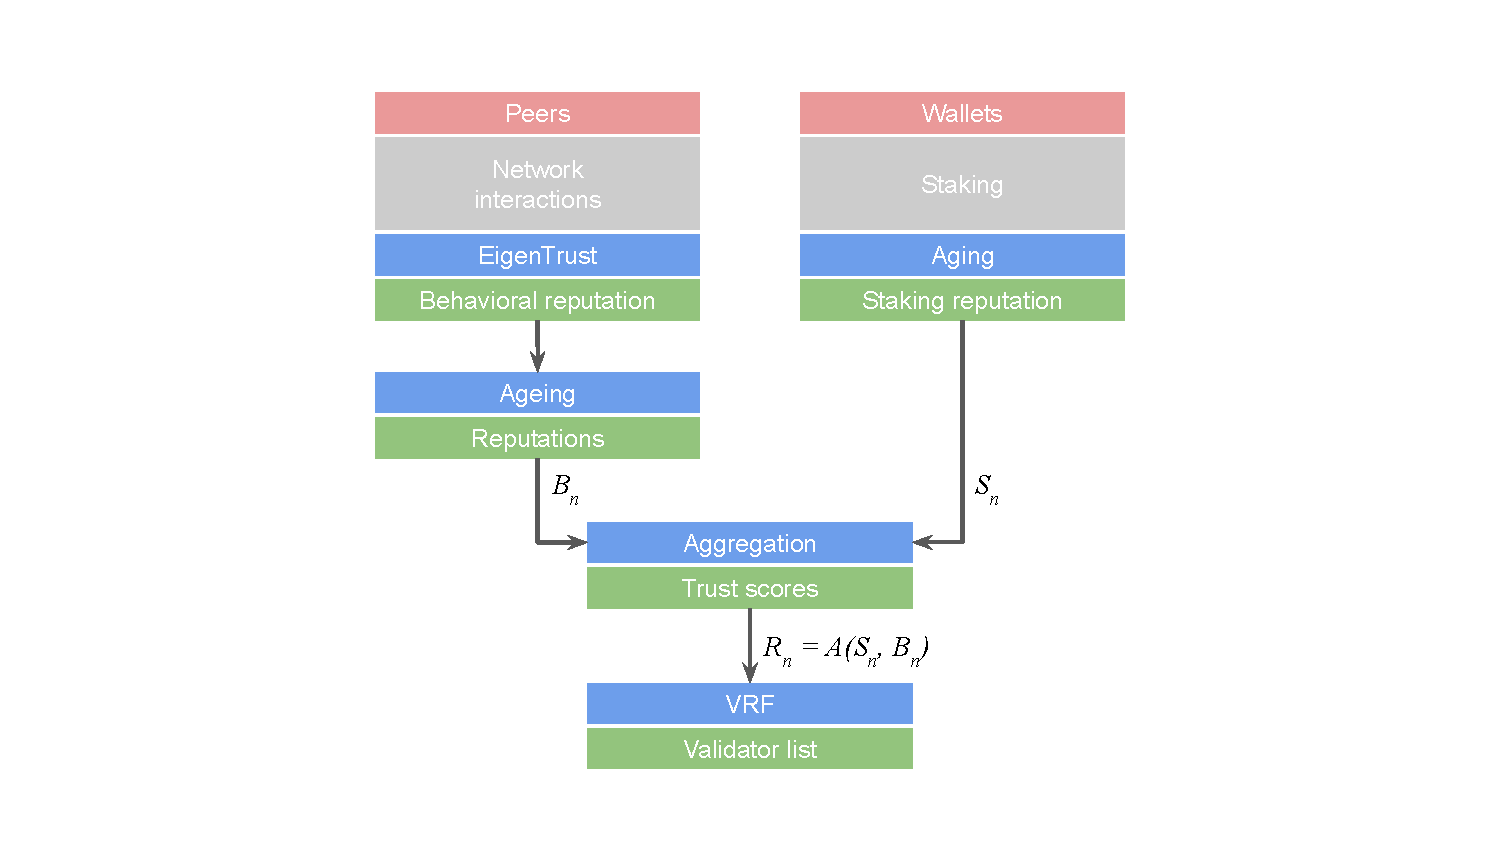
\includegraphics[width=0.6\linewidth, trim= 6cm 0cm 6cm 1cm, clip]{Figures/Overview.pdf}
	\caption{An overview of the PoR validator selection process.}
	\label{fig:overview}
\end{figure}

Figure~\ref{fig:overview} gives an overview of the PoR validator selection process. Each node $n$ in the system is characterised by a reputation constituted of two components. The first is its stake $S_n$ which groups both their own stake and the stakes delegated to them by the community. The second is its trust, which we also call behavioral reputation and denote $B_n$. $B_n$ reflects the honesty of the node in the validation process and its reliability in terms of availability and network level performance. The selection workflow consists then of 2 steps: (i) computing the reputation of the nodes i.e., their trust and stake, and (ii) applying, at each validation round, a random selection to select among eligible nodes those that should participate in that round.  An eligible node is a node with a sufficiently high reputation score. 
To keep it fully decentralized, the random selection is performed through a distributed Verifiable Random Function (VRF) computation during which each node can discover in a secure manner whether it should participate to the validation round or not.  

\subsubsection{Block Validation}
\label{sec:components:blockval}
At the beginning of a validation round, the validators in the elected list are sorted pseudo-randomly to determine their order in the  block validation. Each validator, at its turn, receives the uncofirmed transactions from the other nodes in the system, validates them, includes them in a block, signs the block and broadcasts it to be voted on by the validator list. The block is then confirmed and committed to the blockchain when it reaches the absolute majority of the validator votes.      

\section{Behavioral reputation}
\label{sec:behavior}

\subsection{Trust computation}
As we described in Section~\ref{sec:components:valsel}, the validators are selected, in part, based on their trust in the system. This trust reflects their performance in terms of P2P communication, their availability and their reliability in terms of produced block correctness. In this section, we detail the process of assessing these aspects and the way of computing a glocbal trust score for each node in the netwrok.   

\subsubsection{The EigenTrust algorithm}
The EigenTrust algorithm~\cite{kamvar2003eigentrust} is a distributed trust computation algorithm for Peer to Peer networks. It aims at computing, for each node in a network, a global trust value from the local trust vectors of each peer in this network. It operates as follows: each node rates the communications with its neighbors\footnote{A neighbor is a peer with whom a direct interaction has occurred at least once in the past.}. The node asks its neighbors about their opinions on their neighbors. The node weighs the neighbor opinions by their local weights (i.e. the opinion of the node itself about these neighbors) and combines its opinion and the neighbor opinions to constitute a larger (beyond neighborhood) view of the network. When every nodes performs this computation with multiple hops (asking the neighbors and their neighbors and so on), the system converges for the same full view of the network. This allows to construct in a distributed manner a vector that contains the global trust of each node in the system. That is, how trustworthy a node is from the perspective of the whole system and not only its neighbourhood.

 Formally, it the EigenTrust model, each node $i$ computes a normalized local trust value $c_{ij}$ for node $j$ based on their direct interactions. Then, node $i$ calculates a reputation metric for indirect neighbor, $k$, by asking each neighbor, $j$, for their opinions of $k$ and weighting those opinions by $i$’s opinion of $j$. The trust given by $i$ to $k$ can be then formulated as follows: 

\begin{equation}
 t_{ik} = \sum{j} c_{ij}\times c_{jk}
\end{equation}

Let $C$ be the matrix of reputations $[c_{ij}]$ and Let $\vec{t_i} = t_{ik} \forall k$. The trust vector $\vec{t_i}$ can be expresses as : 

\begin{equation}
   \vec{t_i} = (C^T) \times \vec{c_i}. 
\end{equation}

A node can broaden its view of the system further by asking its neighbor’s neighbor’s opinion. That is $(C^T)(C^T)$. If the node continues in this manner, it will have a complete view of the network after
$n$ iterations. The trust vector $\vec{t_i}$ can then be expresses as : 

\begin{equation}
   \vec{t_i} = ((C^T)^n) \times \vec{c_i}. 
\end{equation}

if $n$ is large, the trust vector  $\vec{t_i}$ will converge to the same vector $\vec{t}$ for every peer $i$. Namely, it will converge to the left principal \textit{eigenvector} of $C$. In other words, $\vec{t}$ is a global trust vector in this model. Its elements, $t_j$ , quantify how much trust the system as a whole places peer j.

\subsubsection{The limitations of EigenTrust}
In order to bootstrap the system and ensure that the reputation computation will not be over taken by a set of malicious nodes, the EigenTrust algorithm relies on a set of pre-trusted nodes, whose "opinions" is accounted for in the computation of the trust of any node in the system. That is, instead of computing the trust of the nodes by only relying on the opinions of the neighbors, their neighbors, etc, a node systematically includes the opinions of a set of pre-trusted nodes in its computation. That is, lets assume that the pre-trusted nodes holds a truste vector $p$ each i.e., how far they trust each node in the system. Then, at each computation iteration k, the trust vector $\vec{t}^{(k)}$ is equal to : 

\begin{equation}
   \vec{t}^{(k)} = (1 - a)(C^T) \times t^{(k-1)} + a \times \vec{p}.
\end{equation}

Where $a < 1$. This is indeed a centralization factor that cannot be accepted in a blockchain where the validation process partially relies on the trust computation (through the validator list selection). We remedy to this limitation by substituting the pre-trusted node by the list of top-$k$ trusted validators of the validator list at each round. 

Furthermore, in its original version, the EigenTrust has been presented as a centralized algorithm where a central authority computes and disseminates the reputation of each node. The authors, however, argued that this is not ideal in a distributed architecture (which is even more true in a blockchain system) and proposed a distributed version of EigenTrust in which each node computes it own reputation. This, however, represents a high security flaw as the network relies on self computed trust which can be easily altered without being detected. Therefore, the authors settled on using Distributed Hash Tables (DHT) to cryptographically distribute the node trust computation and create a system where one node compute the trust of another node (or multiple other nodes). Coupled with redundancy, this allows a more secure trust computation and dissemination. This however adds additional complexity to the system for maintaining the DHT structure and its routing. More over, this is useless in a system such as the blockchain, where a distributed validated state is present in the system exists at any moment. Therefore we propose to use self computed trust with a validation and dissemination process similar to the block validation process. Formally, each peer can compute its own global trust value:

\begin{equation}
   \vec{t}^{(k)}_i = (1 - a)(c_{1i}t^{(k-1)}_1 + ... + c_{mi}t^{(k-1)}_m)  + a\vec{p_i}
\end{equation}

\subsection{Trust features}
The behavioral features that reflect the trust of a node - and wich allows to compute the values of $c$ - are inferred in the system on four levels: the network level, the blockchain logic level, the administration level and the reputation system level. (i) Network level features are common between all distributed architecture. They encompass physical failures such as timeouts, high latency and missed packets. (ii) The blockchain level features relate to the computational and decision making duties of a node. They encompass failures such as delayed block production, and violations such as validating bad transaction and blocks. (iii) The administration level  features reflect the reliability of the human administration of a node. Failing in updating the node in reasonable delays, for instance, can have a negative impact on the performance of the blockchain and is measured as part of the node trust. And finally, (iv) the reputation system features relate to the reputation computation and dissemination duties of the node. They encompasses violations such as reporting wrong or delayed reputation scores \footnote{details on the reputation computation are provided further in this document.}. Table~\ref{tab:violations} lists a set of the features that are taken into account in the node trust computation.

\begin{table}[]
\centering
\begin{tabular}{|l|l|p{7cm}|}
\hline
Level                           & Behavior              & Description                                                \\ \hline
\multirow{3}{*}{P2P}            & High latency          & Latency in answering P2P queries                           \\ \cline{2-3} 
                                & Node timeout          & Number of timeouts, Duration of timeouts                   \\ \cline{2-3} 
                                & Timeout after update  & Timeout in Specific Regime                                 \\ \hline
\multirow{4}{*}{Blockchain}     & Invalid version       & A node running an outdated version                         \\ \cline{2-3} 
                                & Too many requests     & -                                                          \\ \cline{2-3} 
                                & Forks                 & Number of times a node trie to initiate a fork             \\ \cline{2-3} 
                                & No common block       & The node is on another chain                               \\ \hline
\multirow{2}{*}{Administration} & Time to update        & Time after the first none seed node update                 \\ \cline{2-3} 
                                & Public API            & Public API availability                                    \\ \hline
\multirow{3}{*}{Reputation}     & Bad reputation report & A node self reports an invalid reputation score            \\ \cline{2-3} 
                                & No reputation report  & A node does not report its reputation during report period \\ \cline{2-3} 
                                & Bad VRF computation   & A node reports a bad VRF output                            \\ \hline\end{tabular}

\caption{Failures and violations taken into account in the node trust computation.}
\label{tab:violations}
\end{table}

Two things are worth noting in regards of these failures and violations. First, they are not all equally important. Therefore, they are given different numerical values during the trust computation. Indeed, Determining the exact importance factors is a tedious task. It can be achieved through both simulation and real world testing. Second, after specific events such as system upgrade, nodes fall into a specific regime that tolerates some failures such as timeouts and latencies. That is because, when nodes are not all at the same version, the system might be unstable which creates unintentional failures.  

\subsection{Trust aging}
Naturally, during a node's lifetime, failures and violations can either be perpetrated intentionally due to a malicious goal of the node administrator, or accidentally, due to failures in the underlying hardware, software or network. Accordingly, on one hand, the trust computation needs to tolerate some failures by forgetting them if not repeated as they could be accidental. On the other hand, for security reasons, the computation needs to be able to account for each new violation as if it was a malicious one. Therefore, we propose to use exponential history compression~\cite{srivatsa2005trustguard} in order to keep track of all the node behaviour history while giving higher importance for newer infractions and lower importance for older ones. Besides its adaptive accountability advantage, this allows to store the whole trust history in a manageable size vector.   

The history compression allows higher tracking granularity for recent interval which reflects higher importance for recent behaviors and lower granularity for old intervals which reflects lower accountability for older behavior. Its process can be summarized as follows: the behavior history is split into time intervals of size $t$ each. Super-intervals are created by combining the $t$-sized intervals in an exponential manner starting by a super-interval of size 1 grouping the most recent interval. Then a super-interval of size 2 for the second and third most recent intervals and so on. In other words, intervals are of size $2^m$ where $m \geq 0$ determines the history epoch to consider. Figure~\ref{fig:historyComp}, depicts an example of the history compression with 5 history epoch. Finally, in each super-interval the reputation scores of the sub-intervals are aggregated.

\begin{figure}[h]
\centering
	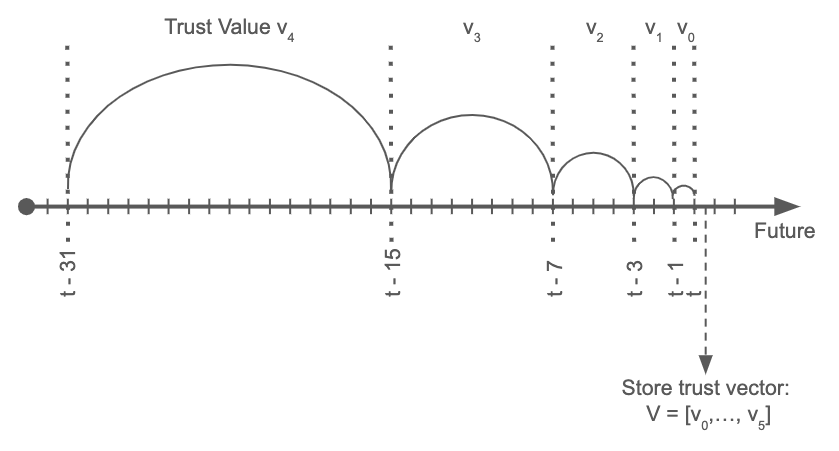
\includegraphics[width=0.65\linewidth, trim= 0cm 0cm 0cm 0cm, clip]{Figures/ageB.png}
	\caption{History slicing and compression for trust age computation.}
	\label{fig:historyComp}
\end{figure}

\begin{figure}[h]
\centering
	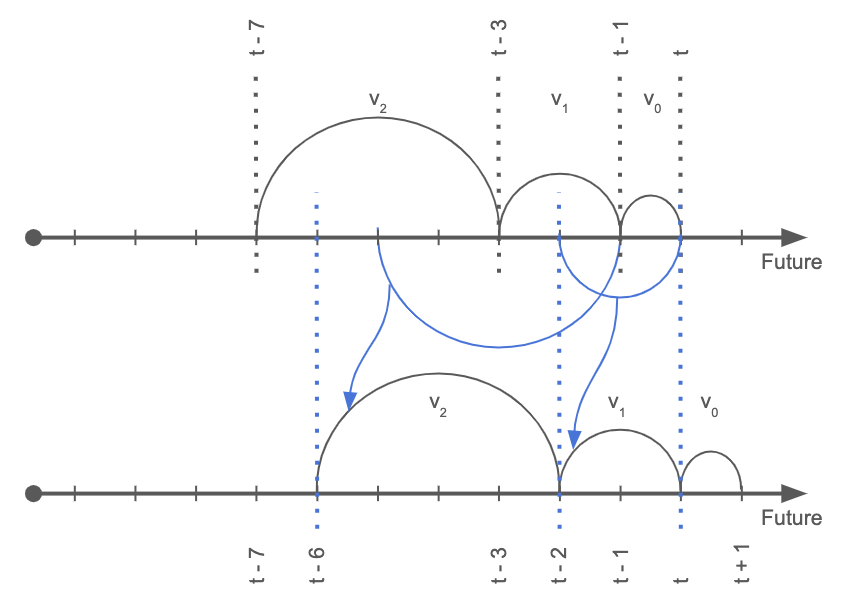
\includegraphics[width=0.65\linewidth, trim= 0cm 0cm 0cm 0cm, clip]{Figures/ageB1.png}
	\caption{An example of aged trust update process.}
	\label{fig:historyCompUp}
	
\end{figure}

In order to update the reputation vector, we adopt a sliding window with an exponential size to merge the trust values within the consecutive intervals. That is, for a super-interval $t$, we estimate the trust value for the sub-interval of size equal to the size of $t+1$ and average it with the trust value of $t+1$. Figure~\ref{fig:historyCompUp} depicts this sliding window computation. Formally:

\begin{equation}
    v^{t+1}[i] = \frac{v^{t}[i] \times (2^i - 1) + v[i - 1]}{2^i}
\end{equation}

The behavioral reputation after ageing is equal to the weighted average of the actual and historical reputation scores of the node. That is, formally : 
\begin{equation}
    \frac{1}{\sum_{k=0}^{m}\alpha_k}\sum_{k=0}^{m}\alpha_k \times v[i - k]
\end{equation}

where $\alpha_k$ is the weight of the reputation for the epoch $k$.\todo{2 times weighting?}  

\subsection{Trust collection and dissemination}
When the reputation of each node is computed and aged, it needs to be disseminated in the network and validated by the current validators. Figure~\ref{fig:disse} depicts the behavioral reputation collection and dissemination process which can be summarized as follows: the runtime is split into reputation epochs. Each reputation epoch is equivalent to a number $K$ of validation rounds. A reputation epoch is defined by one reputation vector i.e., each node has a fix reputation during this epoch. This reputation vector is recomputed before each new epoch to constitute the next epoch's vector. The computation consists of three steps:
\begin{itemize}
    \item Behavior collection: this is a continuous task. The behavior accounted for in the epoch t are collected during epoch t-1 and t-2 during K rounds.
    \item Reputation calculation: Each node computes its own reputation similar to the distributed EigenTrust.
    \item Each node broadcasts its reputation in a specific type of transactions. These reputation transactions are validated by the validator list like any other transactions.
    \item A node that does not broadcast its reputation score during the dissemination period misses its chance to be part in the election process of the next round.
\end{itemize}

The calculation, dissemination and validation occurs in a time window of size $q$ preceding the next epoch.


\begin{figure}[h]
\centering
	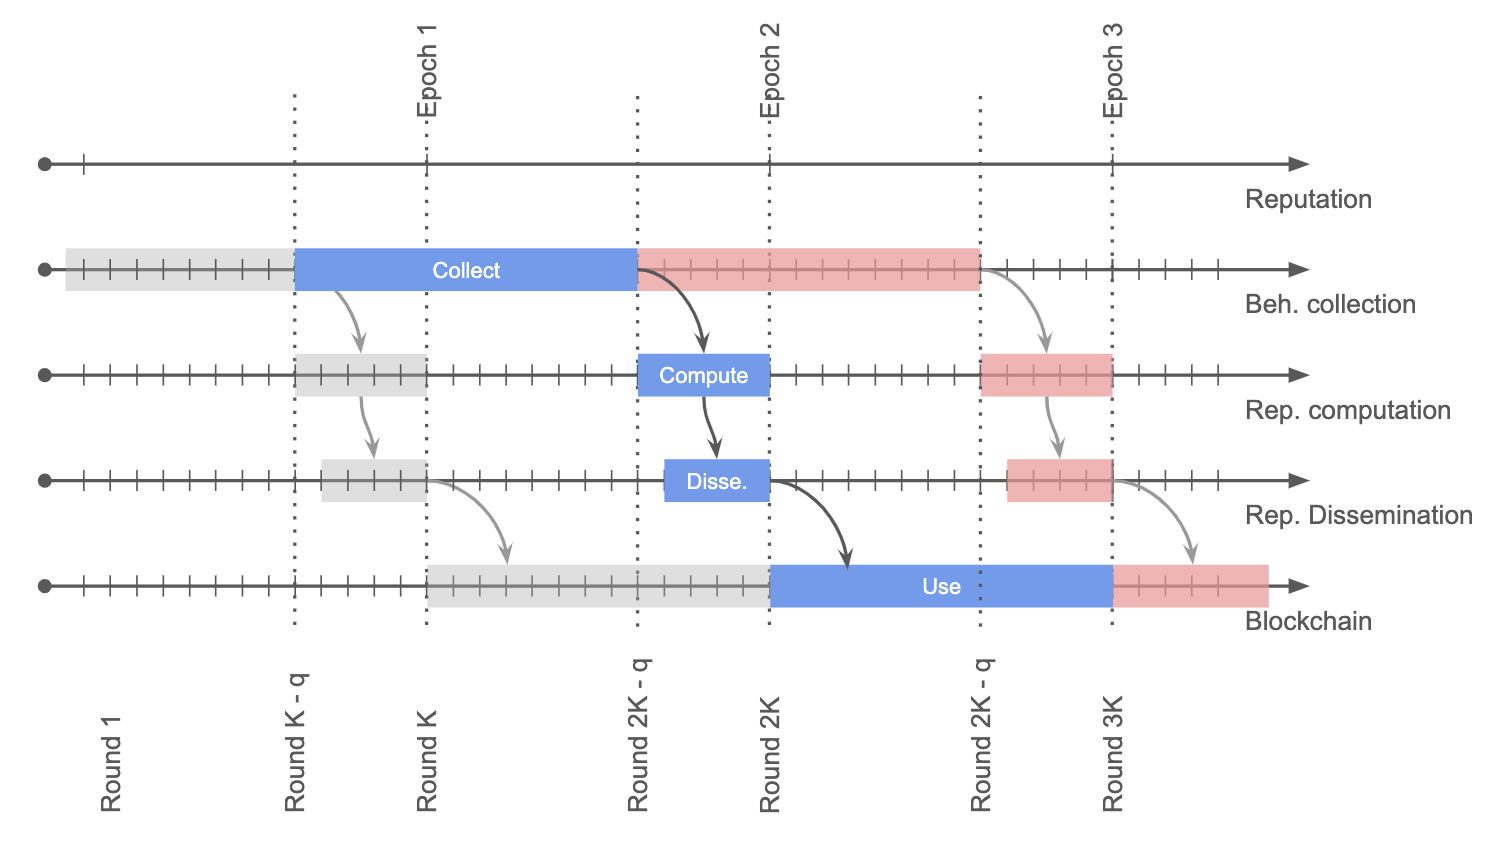
\includegraphics[width=\linewidth, trim= 0cm 0cm 0cm 0cm, clip]{Figures/synch.png}
	\caption{An overview of the trust collection and dissemination epochs}
	\label{fig:disse}
\end{figure}

\section{Staking reputation}
As mentioned earlier, in addition to the behavior of a node, its illegibility to the validation process is determined by the amount of tokens it commits in the system as well as the amount of tokens committed by the wallets who trust and back it to be validating blocks. In this section, we start by describing the wallet scheme and actions and then we detail this illegibility factor which we call the staking reputation.  

\subsection{The Stakeholders}
In the Ki blockchain, a \textbf{stake} is an amount of tokens frozen by their owner in order to show commitment in the system. A frozen token is not spendable unless it is unfrozen first. A \textbf{voter} is a wallet that stakes money to the favor of a validator to improve its chance of being selected in the validation list. An \textbf{owner}, is a wallet that initiates the registration of a validator or inherits the ownership of an existing validator. Tokens staked by an owner wallet represent the validator stake. Slashing, when it occurs, is performed on the token staked by the owner wallet. An owner cannot be a voter as its stake is automatically accounted for the validator they own. Furthermore, a wallet can own one validator only and a validator can be owned by one owner wallet only. Each stakeholder in the system owns two virtual wallets: a hot wallet and a cold wallet. The former contains non frozen tokens that are spendable immediately. The latter contains frozen tokens that are staked and cannot be used unless they are unstaked first. Initially, all tokens belong to the hot wallet. Moving tokens from the hot wallet to the cold wallet, a.k.a. staking, is done through a $freeze()$ function which process is given in the following snippet\todo{All the snippets need to be atomic}:

\begin{lstlisting}[frame=single]
freeze(amount):
    date <- Date.Now();
    this.transfer(this.hot, this.cold, amount);
\end{lstlisting}

\todo{discuss the voting <-> freeze relation}
To unstake tokens, a wallet calls the unfreeze function. In contrast to the freeze function, the effect of the unfreeze is not immediate. It is delayed by a fixed delay to allow reactive accountability on major violation that triggers a slashing event. Indeed by delaying the unfreeze effect, a malicious node cannot spend their staked tokens immediately after a violation to save them from being slashed. The $unfreeze()$ function is shown in the following snippet:

\begin{lstlisting}[frame=single]
unfreeze(amount):
    date <- Date.Now();
    if (amount <= this.cold.balance):
        wait(unfreeze_delay);
        this.transfer(this.cold, this.hot, amount);
\end{lstlisting}

To vote for a validator, a wallet can fall into two cases. First, if the wallet is not already voting for any validator, it broadcasts a voting transaction that contains the amount of token to stake and the validator ID. This transaction performs a $freeze()$ action followed by a voting action in which the system register the vote of the wallet to the indicated validator. The following snippet summarized the process:

\begin{lstlisting}[frame=single]
vote(validator_id, amount):
    date <- Date.Now();
    this.freeze(amount);
    reg_vote(this.id, validator_id);
\end{lstlisting}

Second, if the wallets has already a registered vote then it calls the $switch\_vote()$ function which takes one mandatory parameter that is the new validator ID. 

\begin{lstlisting}[frame=single]
switch_vote(new_validator_id):
    date <- Date.Now();
    if (this.vote != none):
        old_validator_id = this.vote;
        reg_unvote(this.id, old_validator_id);
        reg_vote(this.id, new_validator_id);
\end{lstlisting}

If the wallet decides to stop voting for a validator, it broadcasts an unvote transaction which unfreezes all the cold wallet balance and registers the wallet unvote. 

\begin{lstlisting}[frame=single]
unvote():
    date <- Date.Now();
    if (this.vote != none):
        this.unfreeze(); 
        reg_unvote(this.id);
\end{lstlisting}

When creating a validator a wallet automatically becomes its owner. The registration requires the creation of the validator wallet beforehand. Then the future owner wallet call the $register\_validator()$ function that takes into account the address of the validator wallet as well as the amount of token to stake for it. That is: 

\begin{lstlisting}[frame=single]
create_validator(validator_wallet_id, amount):
    date <- Date.Now();
    this.freeze(amount);
    if (this.validator == none):
        this.set_validator(validator_id)
        this.vote(validator_id)
        reg_validator(validator_id);
    
\end{lstlisting}

For security reasons, a validator administrator needs to be able to transfer the balance of the owner wallet from one wallet to another. This should be made in an atomic swap function that transfers the wallet balance and the validator ownership. Practically, this is a multi-signature transaction as it requires the signatures of the validator node, of the old owner wallet and of the new wallet owner. The $switch\_owner()$ function is called by the old owner who needs to specify the adress of the new owner. The following snippet shows the full ownership swap process.
\todo{Age managment}

\begin{lstlisting}[frame=single]
swap_ownership(new_owner):
    date <- Date.Now();
    ow = this.ID,
    del = this.validator.ID,
    mutlisig_request(ow, del, new_owner);
    while (!all_sig_received):
        wait;
        if (timeout) return;
    reg_swap();
\end{lstlisting}

\subsection{Validator staking reputation}
\subsubsection{formulation}
The staking reputation of a validator is divided into two components: a validator stake and a voter stake. The validator stake is the aged stake of the owner wallet while the voter stake is the aggregated aged stakes of the voter wallets. The validator stake i.e., the stake of its owner wallet, has a greater importance than the voter stake as the former needs to prove a greater commitment in the system. This translates to the followig formulaiton: 

\begin{equation}
\label{eq:stakewalletTypeweight}
    S_n = \alpha\dot{s}_n + (1-\alpha) \sum_{v \in V_n} (\dot{s}_v) 
\end{equation}
where $S_n$ is the staking reputation of the node $n$, $\dot{s}_n$ is the aged stake of the validator, $V_n$ the set of $n$'s voters, $\dot{s}_v$ their aged stakes and $\alpha$ the weight of the validator stake in the reputation such as $0.5 < \alpha <1$. 


\subsubsection{Aging}
While the amount of the stake is an important criteria to measure the confidence and involvement of a stakeholder in the system, this factor is not satisfactory as it does not measure the commitment duration and thus the risk factor accepted by the stakeholder. To explain this statement, we draw the following comparison. Let's consider a wallet $A$ that has frozen a given amount of tokens for a long period of time and a wallet $B$ that alternate between freezing and unfreezing (e.g., for speculation purposes) the same amount of tokens. Let's consider an instant where both wallets have the same stake in the system. It is clear that $A$ has proven a higher commitment in the system than $B$ and thus their stake at the given instant should weigh higher and give $A$ an edge from an eligibility perspective. Therefore we compute the staking reputation of a wallet with respect to its aged stake. That is, the stake weighted by the continuous time (computed as the elapsed time between the current date and the staking date) it spent in the hot wallet. Formally, for a wallet $w$:

\begin{equation}
\label{eq:sdot}
\dot{s}_w = \sum_{s_{wi}}{(Age(s_{wi}) \times s_{wi})}
\end{equation}
where $s_{wi}$ is the partial stake of a wallet such as $\sum s_{wi} = s_w$. In other words, since a wallet can increase its stake by freezing more token at any moment, the total stake of the wallet consists of a partial stakes of different age each. In Equation~\ref{eq:sdot}, $Age$ is a function that normalized the age (in time unit) and returns the stake weight. $Age$ is shown in Equation~\ref{eq:Age}.

\begin{equation}
\label{eq:Age}
    Age(x) = 1 - e^{-kx} 
\end{equation}
Here, $x$ is the age of a stake in natural time unit e.g., day, month, etc. or blockchain equivalent time measure such as block count. $k>0$ is a shaping parameter. The shape of $Age$ for different values of $k$ is depicted in Figure~\ref{fig:Age}. It is interesting to make a set of observations related to this shape and to interpret them in terms of token economics and incentive policies. First, this function tends to 1 without equaling it. This means that the stake is never considered in its totality. However, this constitutes a permanent incentive for wallet to keep the stakes frozen as there is always a room for weight gain, and accordingly, for reputation gain. Second, one can tune $k$ to configure different incentive mechanisms through the speed of weight gain. For instance, larger value of $k$, e.g., $k = 2$, the weight increases strongly during a short time window (90\% of weight reached in one month) which can encourage the wallets to unstake as they can quickly rebuild their reputation. In contrast, lower values of $k$, e.g., $k = 0.1$, induces a very slow weight gain (90\% of weight reached in 24 months) which might discourage wallets from staking large amounts at the first place.       

\begin{figure}[]
\centering
	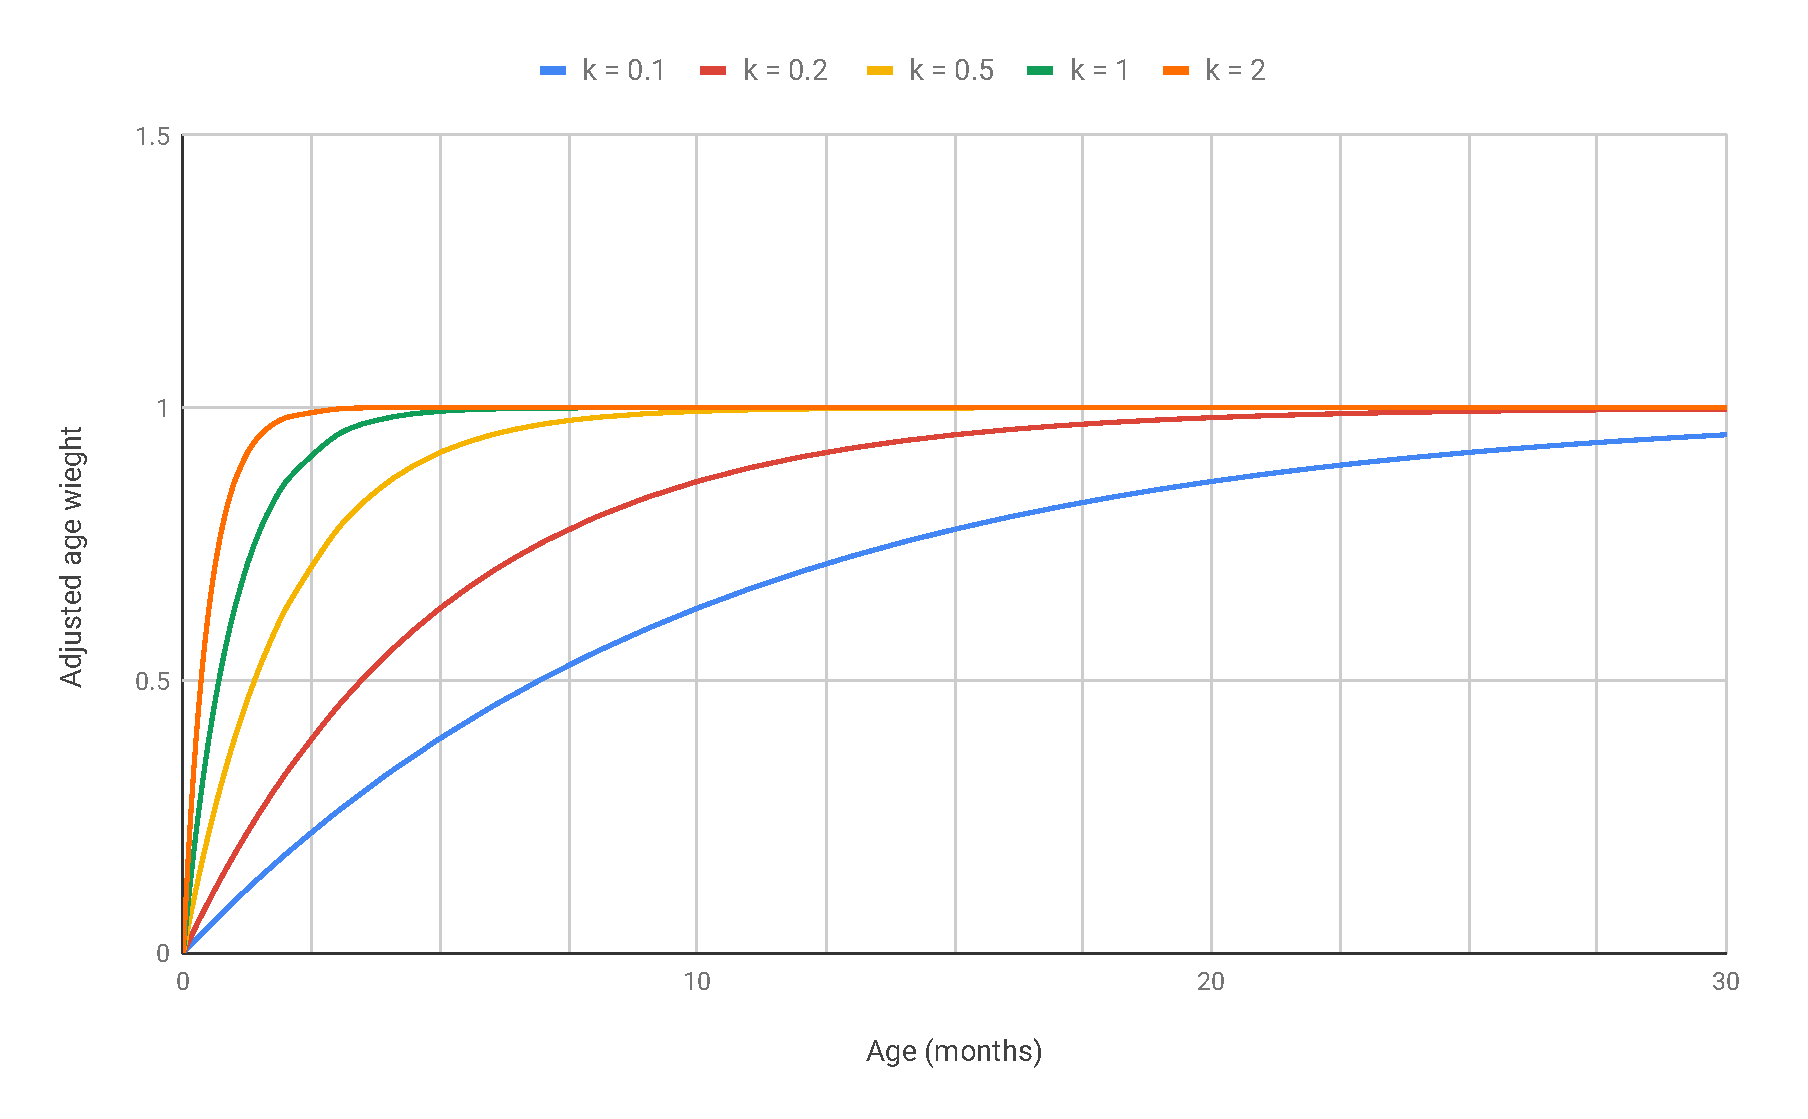
\includegraphics[width=0.9\linewidth, trim= 0cm 0cm 0cm 0cm, clip]{Figures/chart.pdf}
	\caption{The shape of the ageing for different values of $k$.}
	\label{fig:Age}
\end{figure}

% Maximum age: A partial stake gets more weights when it ages gets higher. However this increase in the age value should be bound and must not tend to infinity. In other words, after a set amount of time, the stake reaches its maximum weight of 1 and it remains there until it is unstaked to return to 0.  
			
% This allows to optimize the computation of the total weighted stake. The system can forget (during the computation not stocking) the staking date for token staked before the date where the bound is met. The computation can then be simplified from weighted sum to normal sum.

After applying the aging and weighting w.r.t. the wallet type, the reputation stake $S_n$ of a validator $n$ can be expressed in terms of the various parameters of the system as shown in the Equation~\ref{eq:stakeFinal}. \todo{Normalization?}

\begin{equation}
\label{eq:stakeFinal}
    S_n = \alpha\sum_{s_{ni}}{(1 - e^{-kx_{i}}) \times s_{ni}} + (1-\alpha) \sum_{v \in V_n} \sum_{s_{vj}}{(1 - e^{-kx_{j}}) \times s_{vj}}
\end{equation}


\subsubsection{Age loss}
vThe partial stakes $s_{wi}$ of a wallet $w$ are stored in a FIFO structure. When a wallet unfreezes a given amount, tokens that are removed from their stake are the older ones in this stake. In other words, unstaking removes the tokens with the highest staking weight. We illustrate this with the following example. Assume that $Alice$ is a Ki wallet owner in the system. The staking history of $Alice$ is stored in the data base as a vector of $(stake, date)$ tuples. Table~\ref{tab:stakeex} shows an example series of staking events and their effect on the $Alice$'s staking vector.

\begin{table}[]
\centering
\begin{threeparttable}
\begin{tabular}{|l|p{8cm}|}
\hline
Event & Staking Vector \\
\hline
S, 10, t0 = 10/10/2019 & [(10, t0)]\\
S, 20, t1 = 11/10/2019 & [(10, t0), (20, t1)]\\
U, 25, t2 = 20/10/2019 & [(0, t0), (5, t1)]\\
S, 60, t3 = 22/10/2019 at 6pm  & [(0, t0), (5, t1), (60, t3)]\\
S, 20, t4 = 22/10/2019 at 9pm & [(0, t0), (5, t1), (60, t3), (20, t4)]\\
U, 20, t5 = 15/11/2019 & [(0, t0), (0, t1), (45, t3), (20, t4)]\\
U, 10, t6 = 16/11/2019 at 8am & [(0, t0), (0, t1), (35, t3), (20, t4)]\\
S, 40, t7 = 16/11/2019 at 6pm & [(0, t0), (0, t1), (35, t3), (20, t4), (40, t7)]\\
S, 50, t8 = 10/12/2019 & [(0, t0), (0, t1), (35, t3), (20, t4), (40, t7), (50, t8)]\\
S, 60, t9 = 25/12/2019 & [(0, t0), (0, t1), (35, t3), (20, t4), (40, t7), (50, t8), (60, t9)]\\
\hline
\end{tabular}
\begin{tablenotes}
\centering
      \small
      \item Event : Stake (S) or Unstake (U), amount, date.
    \end{tablenotes}
 \end{threeparttable}
 \caption{An example of staking events and the FIFO scheme.}
\label{tab:stakeex}
\end{table}

Since it can be easy to flood the database with micro stakes we define 3 rules for the staking. First, a minimum stake amount is required. Second, fees on staking applies starting the second stake per day. Finally, the staking events of are compressed on a daily basis. This means that all the staking actions are aggregated in one day and than committed to the database daily. On the other hand, unstaking events take effect immediately \footnote{ To simulate the staking and unstaking events and the stake vector computation, an online tool has been created and made public on \url{https://static.foundation.ki/blockchain/stake-demo/index.html}.}. If one applies this third rule on $Alices$ events, her final staking vector will be equal to: 

\begin{lstlisting}[frame=single,  basicstyle=\small]
[(55, 22/10/2019),(40,16/11/2019),(50, 10/12/2019),(60, 25/12/2019)]
\end{lstlisting}
This vector serves as an input for the stake reputation function shown in Equation~\ref{eq:stakeFinal}.

\subsubsection{Role switching}
From a staking perspective, a wallet can switch from being a normal voter to an owner wallet (i.e., indirectly possessing a validator stake weight) and vice versa. Indeed, since the type of the wallet impacts its stake weight (See Equation~\ref{eq:stakewalletTypeweight}), it is important to define rules to0 account for these transitions. On one hand, one can reset the age of the token to 0 when the wallet type changes. On the other hand, one can perform a detailed computation of the stake by taking into account the weight of the stake according to the wallet type at the staking date. The former solution is extremely unfair as it completely deprives the wallet from their age. The latter, while optimally fair, is costly from a computation point of view. In the Ki blockchain, we chose a practical and faire trade-off between these 2 possibilities. In fact, as long as the stake is continuous (i.e., the wallet did not unstake during the transition), its age - in time units - is conserved in its totality. Its weight in the  staking reputation of the validator they own or vote for, is computed w.r.t. the current state of the wallet (i.e., whether it is a voter or an owner at the moment of computation). For the purpose of comparison, an example where the three solutions are detailed can be found in the followinf url: \url{https://raw.githubusercontent.com/KiFoundation/ki-yellowpapers/master/KIYP3-PoR/Figures/roleswitch.svg?sanitize=true}.

\section{Validator list selection}
As mentioned in Section \ref{sec:overview}, at each reputation round the reputation of the validators is updated. This means that the behavioural reputations, $B_n$, is recalculated based on the last observations of the nodes and the stake reputations, $S_n$, are recalculated based on the latest staking, unstaking and voting events. $B_n$ and $S_n$ are then aggregated using a linear combination to yield the eligibility scores $R_n$ as shown in Equation~\ref{eq:aggregation}. 

\begin{equation}
\label{eq:aggregation}
    R_n = \omega_S \times S_n + \omega_B \times B_n
\end{equation}
where $\omega_S$ and $\omega_B$ are the weights of the staking and reputation score respectively. The values of these weights are discussed further in this document. Obviously, a lower reputation score reflects the unreliability of a node and its lack of commitment. Nodes with lower scores are not allowed to participate to validation as they represent a security risk. Therefore we split the pool of validators into eligible and non eligible validators based on a given threshold $\rho$. Among the eligible node a distributed and secure random selection process is performed at each validation round to select the list of validators for that round. 

The random selection process relies on a Verifiable Random Function (VRF) computation. In a nutshell, a VRF \cite{micali1999verifiable,dodis2005verifiable} is a function that allows a party to compute the hash of a given value and to produce, using their private key, a cryptographic proof that can be used by other parties to verify the correctness of this computation using the public key of the proof generating party. The selection process can be summarized as follows: each node $n$ is characterized by an interval $[0, P_n]$ relative to its reputation score in the system. Each node $n$ has also a private key $K_n$ and public key $pK_n$ dedicated to the Verifiable Random Function (VRF) computation. At each round a random seed $Q$ is disseminated on the network (e.g., last block hash). Each node computes the $VRF(K_n, Q)$ which yields a couple $(V_n, proofV_n)$ where $V_n$ is the unique possible output of the VRF for each input couple $(K_n, Q)$. $ProofV_n$ allows everyone to verify the correctness of the $V_n$ using the $pK_n$ of the correspondent node. Finally, a node participates in the next round of validation if and only if $V_n$ belongs to $[0, P_n]$. The larger the interval is, the more reliable a node is and the higher their chances of being selected are. \todo{How to be restrict the number of selected nodes}

\section{Reputation epochs}
\label{sec:epochs}
Reputation epochs allows to adapt the configuration of the reputation system to the evolution of the blockchain validation activity i.e. number of validators, the distribution of their reputation values, ... The epoch duration and configurations are defined through the governance process, they encompass: the size of the eligible pool, the minimum eligibility reputation, the size of the round validator list, the weights of the global reputation formula (stake, behavior), the weights of the stake reputation components (owner/voter stakes).

\section{Summary}
\label{sec:conclusion}
In the document we described the Proof of Reputation consensus protocol. In order to ensure the reliability of the nodes, the PoR protocol leverages both, the trust of these nodes measured by their behavioural features and their staking reputation measured by the aggregate of their aged stake and the aged stake of their voters. This compound commitment score guarantees the security of the validation process as only technically reliable nodes are selected. Moreover the proposed random validator selection mechanism ensures a high level of decentralization as reliable nodes can be selected regardless how wealthy they. 



\bibliographystyle{unsrt}
\bibliography{biblio}

\end{document}
